\section{Deep Q-Learning}

\subsection{Introduction}

\begin{figure}[h]
	\centering
	
	\begin{subfigure}{.3333\textwidth}
		\centering
		\includegraphics[width=4cm]{cartpole.png}
		\caption{}
		\label{fig:cartpole}
    \end{subfigure}%    
    % 
    \begin{subfigure}{.3333\textwidth}
		\centering
		\includegraphics[height=2.5cm]{breakout.png}
		\caption{}
		\label{fig:cartpole}
	\end{subfigure}%
	
	\caption{Shown are two examples of environments, Deep Q-Learning can be used for. (a) Cartpole (b) Atari Breakout game}
	\label{fig:examples}
\end{figure}

The question arises, how to train an agent in a complex environment, that reacts to the agents actions. Examples for such an environment are games like Atari-Breakout or the cartpole example.
\\
\\
It is not easily possible to provide training data for decision making, because the decision and the result may be remote in time from each other. One way to address such an problem is Deep Q-Learning. This algorithm was proposed in 2013 by Google DeepMind \cite{DQN} and has successfully been applied to several Atari-Games. Deep Q-Learning is an extension of Q-Learning. To introduce Deep Q-Learning I will first provide an formalisation of such an environment, then introduce Q-Learning and extend it to Deep Q-Learning. 
\\
\\
To apply this algorithm, the world is modelled as Markov-Decision-Process. The environment is represented as state vector $s_i$. Considering the state $s_i$ the agent can choose a certain action $a_i$. Actions transform the state and may lead to a reward $r_i$. A Markov-Decision-Process may be stochastic, denoting that the state resulting from taking a certain action in a certain state is not deterministic. The set of states, corresponding actions and rules for transitioning between these states and for getting rewards form the Markov-Decision-Process. 
\\
\begin{figure}
	\centering
	\begin {tikzpicture}[auto]
		\node[draw, circle] (agent) at (0,1.5) [] {agent};
		\node[draw, rounded corners, minimum width=40pt, minimum height = 20pt] (environment) at (0,0) {environment};
		\path [draw, ->] (environment) 	to [out=190, 	 in=180] 				node {state, reward} 		(agent);
		\path [draw, ->] (agent) 				to [out=350,     in=0] 					node {action} 					(environment);
	\end{tikzpicture}
    
	\caption{Reinforcement Learning problem}
	\label{fig:refprob}
\end{figure}


One episode of a Markov-Decision-Process leads to a chain of consecutive states, actions and rewards: 
$s_0, a_0, r_0,  s_1, a_1, r_1,  s_2, a_2, r_2, ..., s_n, a_n, r_n, $
\\
\\
The expected value of an action can not be measured by simply summing up all expected future rewards, because a Markov-Decision-Process is stochastic. Thus it can not be guaranteed, that the states visited during one episode are always the same. The uncertainity, that the expected reward and the actual reward diverge grows, the further the decision is away in time. An appropriate tool to measure the value of an action is expected discounted future reward. Here $\gamma$ is called discount factor, denoting how much reward \textit{discounts} over time.

\begin{equation*}
R_t = r_t + \gamma * r_{t+1}  +  \gamma^2 * r_{t+2}   +   ...   +    \gamma^{n-t} * r_{t+n}. 
\end{equation*}


% Introduce Q-Learning (Q-Table, Policy, Bellman Equation)
\subsection{Q-Learning}

Q-Learning is an algorithm to learn a policy to determine the best action for every state. A function $Q(s, a)$ is defined. This function will be trained to represent the discounted reward for every state action-pair. Using this function the policy $\pi$ determines the best action for every given state, by choosing the action with the expected highest discounted reward:

\begin{equation*}
\pi(s) = argmax_a Q(s, a).
\end{equation*}
\\
To train the $Q$ function, the algorithm can iteratively consider multiple transitions in the Markov-Decision-Process $(s, a, r, s')$ and update the Q-function acording to the Bellman-Equation:

\begin{equation*}
Q(s, a) = r + \gamma * max_{a'}Q(s', a').
\end{equation*}
\\
The idea behind this equation is, that the $Q$-Fuction will hold the true expected future discounted reward, if it has been updated with enough transitions. 
\\
\\
The final algorithm lets the agent learn in its environment by executing multiple actions and observing the transitions: 
\\
\\
\begin{algorithm}[H]
	\KwData{ rules for Markov decision process, number of training episodes $E$, learning rate $\alpha$ }
	\KwResult{ trained Q-Table }
	\For{ $i$ from $1$ to $E$ } {
		$ s \leftarrow $ observe initial state \\
		\While{ not terminated } {
			$ a \leftarrow \pi(s) $	\\
			$ r, s' \leftarrow$ carry out a and observe reward and new state 		\\
			\eIf { environment not terminated } {
				$ Q(s, a) = Q(s', a') + \alpha * (r + \gamma * max_{a'}) $
			} {
				$ Q(s, a) \leftarrow r $
			}
			$ s \leftarrow s' $
		}
	}
\end{algorithm}
~\\
\\
Applying this algorithm to the cartpole example may lead to the following exemplary Q-Table. The state vector of the cartpole example contains of the cartpoles current x position, the previous x position, the current pole angle, the previous pole angle.: 
\\
\begin{table}[h]
  \centering
  \begin{tabular}[c]{llc}
    \hline
    $s_i$												& $a$ 		& 	$Q(s, a)$				\\
    \hline
    $(2.32, 2.29, 0.14, 0.16)$ 				& Right 	& $0.132 $  			\\
    $(1.21, 1.24, 0.19, 0.11,)$ 			& Left 	& $0.442$   				\\
    $(0.03, 0.12, 1.47, 1.59)$ 				& Right 	& $0.842$   				\\
    ... 																& ...			& ... 				\\
    \hline
  \end{tabular}
  \caption{Extract of exemplary Q-Table}
  \label{tab:qtable}
\end{table}


\subsection{Deep Q-Learning}

Applying Q-Learning to complex states like the raw graphical input of an Atari-Game is nearly impossible, because the number of possible states and thus the entries to the Q-Table grows very quick. One solution to this problem is using an neural network, called Q-Network, to approximate the Q-Table. Neural networks have proven to work very well on highly structured data, like image data. In the original paper a neural network has been used to approximate the Q-Table. The algorithm achieved human level results on several Atari-Games. In the following I will introduce the Deep Q-Learning algorithm and the show practical results applying it to the Breakout-Game and cartpole example. 

\subsubsection{Q-Network}

The Q-Network takes the state vector as input and outputs expected discounted future reward for every possible action. The network structure is shown in the following figure:
\\
\begin{figure}[h]
	\centering

	\tikzstyle{input}=[draw, circle, minimum size=19pt, inner sep=0pt]

	\centering
	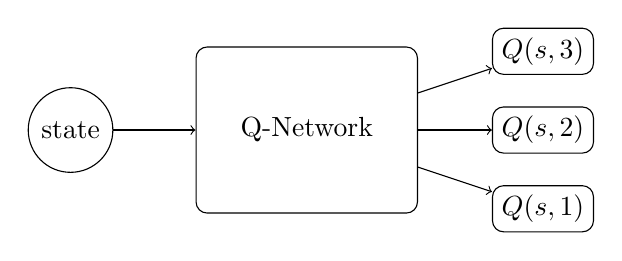
\begin{tikzpicture}
	
		\node[draw, circle, minimum size=20pt] (state) at (0,0)    {state};
		\node[draw, rounded corners, minimum width=80pt, minimum height=60pt] (qnet) at (3,0) 	{Q-Network};
		
		\node[draw, rounded corners] (q1) at (6,-1) 		{ $Q(s, 1)$ };
		\node[draw, rounded corners] (q2) at (6,0) 		{ $Q(s, 2)$ };
		\node[draw, rounded corners] (q3) at (6,1) 		{ $Q(s, 3)$ };
		
		\draw [->] (state) -- (qnet);
		\draw [->] (qnet) -- (q1);
		\draw [->] (qnet) -- (q2);
		\draw [->] (qnet) -- (q3);
			
	\end{tikzpicture}
	\caption{Input and Output structure of Q-Network}
	\label{fig:qnet}
\end{figure}

Given an transition $(s, a, r, s')$ the Q-Network is trained to predict the new value for the action: 

\begin{equation*}
y = r + \gamma * max_{a'}Q(s', a').
\end{equation*}
\\
The network is trained doing a backpropagation step on $(y - Q(s, a))^2$.

\subsubsection{Experience Replay}

To achieve better training results the visited transitions are stored in the so called replay-memory. Every step a batch of this replay-memory is sampled. The Q-Network is then trained using this batch. This approach results in better training results, because each step is potentially used in multiple weight updates. Furthermore multiple consecutive transitions may have strong correlation. Randomizing the samples breaks these correlations and avoids the agent to get stuck in a local minimum. If the correct action for the agent may be to turn right for a long period of time the training data will be dominated by such examples. By sampling the transitions from the replay memory, these transitions are spread over multiple batch updates.  

\subsubsection{Exploration}

In Deep Q-Learning the actions choosen initially are random, because the Q-Table is initialized randomly. Thus the agent may stuck in a certain local minimum. To avoid this, the agent "explores" random transitions. In every step with a probability $\epsilon$ the agent chooses a random action. It is common to reduce $\epsilon$ with every training episode to let the agent optimize its strategy after exploration. 

\subsubsection{Final Algorithm}

The final algorithm becomes: 
\\
\\
\begin{algorithm}[H]
	\KwData{ rules for Markov decision process, number of training episodes $E$ }
	\KwResult{ trained Q-Network }

	initialize replay memory $R$ to capacity $M$		\\
	initialize Q-Network $Q$ with random weights		\\	
	
	\For{ $i$ from $1$ to $E$ } {
		$ s \leftarrow $ observe initial state					\\
		\While{ not terminated } {
			With probability $\epsilon$ select random action $a$ 		\\
			Otherwise select action $a$ by executing $\pi(s)$			\\
			$ r, s' \leftarrow $ Carry out a and observe reward and new state	\\
			Sample random minibatch of transitions from $R$			\\
			\For {every transition $(s_i, a_i, r_i, s'_i)$ in minibatch} {
				\eIf {environment not terminated } { 
					$y_i \leftarrow r + \gamma * max_{a_i'}Q(s_i', a_i')$
				 } {
				 	$y_i \leftarrow r_i$
				 }
				 Train Q-Network using $(y_i - Q(s_i, a_i))^2$  \\
			}
		}
	}
\end{algorithm}

\subsection{Practical Results}

\subsubsection{Atari Games}

In the original paper \cite{DQN} Deep Q-Learning was used to play several Atari-Games. The games were emulated by an Atari game emulator which displays the games as 210x160 RGB images at 60 Hz. It is not possible to derive the full game state from one image, because motion information can not be derived. Thus a sequence of consecutive images have to be stacked, to model one state of the Markov decision process. Additionally the images are bascially downscaled to achieve better performance. As Q-Network a convolutional network, consisting of 3 convolutional layers and 2 fully connected layers, is used. Convolutional networks are a special kind of neural networks used for image processing. Convolutional networks used by Deep Q-Learning are referred to as Deep Q-Networks. 
\\
\\
The authors implementation of the Deep Q-Learning algorithm was tested on 7 Atari games. They report, that their method achieves better performance than an expert human player on Breakout, Enduro and Pong and it achieves close to human performance on Beam Rider. The same network architecture and hyperparameters were used across these games. 
\\

\begin{table}[h]
  \centering
  \begin{tabular}[c]{lccccccc}
    \hline
    						& B. Rider 		& Breakout 		& Enduro 	& Pong 	& Q*bert 		& Seaquest 	& S. Invaders			\\
    \hline
    Human			& 7456				& 31					& 368			& -3			& 18900		& 28010			& 3690						\\
    DQN				& 4092				& 168				& 470			& 20			& 1952			& 1705				& 581						\\
    DQN Best		& 5184				& 225				& 661			& 21			& 4500			& 1740				& 1075						\\
    \hline
  \end{tabular}
  \caption{ \cite{DQN} 
  					The upper table compares average total reward for Deep Q-Learning to an expert human player. 
  					The row DQN Best shows the single best performing episode of Deep Q-Learning. }
  \label{tab:comparison}
\end{table}


\subsubsection{Cartpole Example}

% Architecture + Preprocessing + ANN
% Results

I applied my implementation of Deep Q-Learning to the cartpole example. In this 2 dimensional example a pole is attached to a cart, which moves along a track. The goal is to keep the pole standing upright, by moving the cart. An image of the cartpole is shown in Figure \ref{fig:cartpole}.
\\
\\
To simulate the cartpole I used the Python OpenAI Gym, a powerfull toolkit to work with reinforcement learning. My implementation of Deep Q-Learning was written in Python. The Deep Learning library Keras was used to implement the Q-Network. To apply Deep Q-Learning the cartpole model is modelled as Markov decision process. Each state consists of the cartpoles current x position, the previous x position, the current pole angle, the previous pole angle. As Q-Network a feedforward network, consisting of 3 layers with 24 neurons each, was used. As activation function $tanh$ was used. To train the agent minibatches of size 32 were sampled from a replay memory of size 2000, with $\epsilon$ annealed linearly from 1.0 to 0.0 and fixed at 0.0 thereafter. 
\\
\\
I capped the number of possible steps in the cartpole example to 2000 steps, to avoid the training process getting stuck in an infinite loop. The observed average number of steps during 2000 training episodes is shown in Figure \ref{fig:cartpole_result}
\\
\begin{figure}
	\centering
	\includegraphics[width=10cm]{results-cartpole-avg10-2017steps.png}
	\caption{Deep Q-Learning training results for cartpole example}
	\label{fig:cartpole_result}
\end{figure}

As you can see the number of steps does not converge to the maximum of 1000 in a stable way, but the number of steps per episode increases and reaches the maximum several times. As the authors of the original payper state, a problem with Deep Q-Learning is, that small changes to the Q-Network may lead to big changes in the actions taken. 

